\documentclass{beamer}
\usepackage{lmodern}
\usetheme{Copenhagen}
\setbeamertemplate{headline}{}
\newcounter{saveenumi}
\newcommand{\seti}{\setcounter{saveenumi}{\value{enumi}}}
\newcommand{\conti}{\setcounter{enumi}{\value{saveenumi}}}
\usepackage[]{graphicx}\usepackage[]{xcolor}
% maxwidth is the original width if it is less than linewidth
% otherwise use linewidth (to make sure the graphics do not exceed the margin)
\makeatletter
\def\maxwidth{ %
	\ifdim\Gin@nat@width>\linewidth
	\linewidth
	\else
	\Gin@nat@width
	\fi
}
\makeatother

\definecolor{fgcolor}{rgb}{0.345, 0.345, 0.345}
\newcommand{\hlnum}[1]{\textcolor[rgb]{0.686,0.059,0.569}{#1}}%
\newcommand{\hlstr}[1]{\textcolor[rgb]{0.192,0.494,0.8}{#1}}%
\newcommand{\hlcom}[1]{\textcolor[rgb]{0.678,0.584,0.686}{\textit{#1}}}%
\newcommand{\hlopt}[1]{\textcolor[rgb]{0,0,0}{#1}}%
\newcommand{\hlstd}[1]{\textcolor[rgb]{0.345,0.345,0.345}{#1}}%
\newcommand{\hlkwa}[1]{\textcolor[rgb]{0.161,0.373,0.58}{\textbf{#1}}}%
\newcommand{\hlkwb}[1]{\textcolor[rgb]{0.69,0.353,0.396}{#1}}%
\newcommand{\hlkwc}[1]{\textcolor[rgb]{0.333,0.667,0.333}{#1}}%
\newcommand{\hlkwd}[1]{\textcolor[rgb]{0.737,0.353,0.396}{\textbf{#1}}}%
\let\hlipl\hlkwb

\usepackage{framed}
\makeatletter
\newenvironment{kframe}{%
	\def\at@end@of@kframe{}%
	\ifinner\ifhmode%
	\def\at@end@of@kframe{\end{minipage}}%
\begin{minipage}{\columnwidth}%
	\fi\fi%
	\def\FrameCommand##1{\hskip\@totalleftmargin \hskip-\fboxsep
		\colorbox{shadecolor}{##1}\hskip-\fboxsep
		% There is no \\@totalrightmargin, so:
		\hskip-\linewidth \hskip-\@totalleftmargin \hskip\columnwidth}%
	\MakeFramed {\advance\hsize-\width
		\@totalleftmargin\z@ \linewidth\hsize
		\@setminipage}}%
{\par\unskip\endMakeFramed%
	\at@end@of@kframe}
\makeatother

\definecolor{shadecolor}{rgb}{.97, .97, .97}
\definecolor{messagecolor}{rgb}{0, 0, 0}
\definecolor{warningcolor}{rgb}{1, 0, 1}
\definecolor{errorcolor}{rgb}{1, 0, 0}
\newenvironment{knitrout}{}{} % an empty environment to be redefined in TeX

\usepackage{alltt}
%\usepackage{fullpage}
\usepackage{graphicx}
\usepackage[utf8]{inputenc}
\usepackage{amsmath}
\usepackage{graphics}
\usepackage{float}
\usepackage{xcolor}
\usepackage{geometry}
\usepackage{tikz}
\usetikzlibrary{shapes, arrows}
\usepackage[utf8]{inputenc}
\usepackage{amsmath}
\usepackage{graphics}
\usepackage{xcolor}
\usepackage{hyperref}
\usepackage{longtable}
\usepackage{array}
\usepackage{adjustbox}
\numberwithin{equation}{section}
\numberwithin{table}{section}
\IfFileExists{upquote.sty}{\usepackage{upquote}}{}
\title{Modeling Depression Severity among Caregivers in a Rural Setting using Ordinal Logistic Regression}

\author[]{BEVERLY KIND : \hspace{0.2cm}    I63/4240/2019 \\ CHARLES WAMBUA : \hspace{0.2cm}     I63/4248/2019\\ ODHIAMBO KENNEDY : \hspace{0.2cm}    I63/4282/2019\\ PETER DOKTA : \hspace{0.2cm}    I63/136668/2019\\DOMINIC NYAENYA : \hspace{0.2cm}    I63/4261/2019\\ \vspace{0.2cm} \textbf{SUPERVISOR}: DR. MUSIGA}
\institute[]{
\includegraphics[width=0.1\textwidth]{UoN_Logo.png}}
\date{June 28, 2023}
\begin{document}
\maketitle
\section{Introduction}
\begin{frame}{Background information}
\begin{itemize}
	\item Depression is a mental health disorder characterized by persistent feelings of sadness, loss of interest or pleasure in activities, changes in appetite or sleep patterns, fatigue, difficulty concentrating, and thoughts of self-harm or suicide.
	\vspace{4mm}
	\item  Rehabilitation centers for depression have been established to provide specialized treatment facilities that provide comprehensive care for individuals experiencing moderate to severe depression
\end{itemize}
\end{frame}
\begin{frame}{Statement of the Problem}
	$\bullet$ Researchers have been faced with the problem of identifying potential predictors of depression among cancer caregivers.\\
	\vspace{3mm}
	$\bullet$ The problem is to identify and to quantify the important variables linked to depression.
\end{frame}
\begin{frame}{Objective of the Study}
	\begin{block}{General objectives}
		\vspace{0.4cm}
Model depression severity among caregivers in a rural setting using ordinal logistic regression model.
	\end{block}
	\begin{block}{Specific objectives}
	\begin{enumerate}
	\item Identify significant predictors that contribute to depression severity among cancer caregivers in a rural setting
	\item Estimate and interpret the coefficient of the factors leading to depression severity.
	\item Determine and Interpret the odds ratio of the factors affecting depression severity.

\end{enumerate}
	\end{block}
\end{frame}
\begin{frame}{Justification of the Study}
	\begin{itemize}
	\item  This study informs healthcare professionals and support groups on targeted treatments for cancer caregivers by identifying the predictors of depression
	
\end{itemize}
\end{frame}
\section{LITERATURE REVIEW}
\begin{frame}{Literature Review}
\begin{enumerate}
	\item Jain et al. (2013);
	\begin{itemize}
	\item  Examined the burden of depression on work productivity in the US workforce among 1051 full-time employees in February 2010.
	\item All levels of depression were associated with decreased work productivity as severity increased, presenteeism and absenteeism worsened.
	\end{itemize}

\item Serpa et al. (2014);

\begin{itemize}
\item Investigated the major problems among Veterans specifically anxiety, depression and suicidal ideation among 79 veterans at an urban Veterans Health Administration medical facility. 
\item The results indicated significant reductions in anxiety, depressions, and  suicidal ideation after MBSR training as well as improved mental health functioning scores although pain intensity and physical health functionality did not register improvements
\end{itemize}
\seti
	\end{enumerate}
\end{frame}
\begin{frame}{Literature Review Cont...}
\begin{enumerate}
	\conti
	\item Laing and Jones (2016)
\begin{itemize}
\item  Investigated the mediation effect of anxiety and depression on the relationship between perceived health-promoting workplace culture and presenteeism among 4703 state employees.
\item  Correlational analysis indicated that indirect effects of workplace culture on productivity, mediated by anxiety and depression symptoms were significant. Healthy living culture and anxiety were significantly negatively associated and anxiety and presenteeism were significantly positively associated.
\end{itemize}
\item Magtibay et al. (2017)
\begin{itemize}
	\item assessed the efficacy of blended learning which was intended to decrease stress and burnout among nurses through the use of the SMART program.
	\item  The results indicated statistically significant, clinically meaningful decreases in anxiety, stress, and burnout and increases in resilience, happiness, and mindfulness.
\end{itemize}
\seti
\end{enumerate}
\end{frame}
\begin{frame}{Literature Review Cont...}
	\begin{enumerate}
		\conti
		\item Levis et al. (2019)
		\begin{itemize}
			\item Evaluated the accuracy of the Patient Health Questionnaire-9 (PHQ-9) for screening major depression in adults using individual participant data meta-analysis.
			\item The study found that combined sensitivity and specificity was maximized at a cut-off score of 10 or above among studies using a semi-structured interview. Secondly across cut-off scores of 5-15, sensitivity with semi-structured interviews was 5\%-22\% higher than for fully structured interviews.
		\end{itemize}
	\item Leung et al. (2020)
	\begin{itemize}
		\item Investigated the factor structure, reliability, and construct validity of the Patient Health Questionnaire-9 (PHQ-9) in a community sample of 10,933 Chinese adolescents.
		\item The results indicated that a one-factor model with three pairs of items correlations fitted the PHQ-9 data well and that measurement invariances by age and gender were supported. The PHQ-9 was also strongly correlated with anxiety, self-esteem and perceived control.
	\end{itemize}
	\seti
	\end{enumerate}
\end{frame}
\begin{frame}{Literature Review Cont...}
	\begin{enumerate}
		\conti
		\item Lister et al. (2023)
		\begin{itemize}
			\item conducted a qualitative study that investigated the barriers and enablers to mental wellbeing and academic success that students experienced in distance learning.
			\item The study found that barriers and enablers were existent in the majority of themes, implying that different aspects of study could be both barriers or enablers for mental wellbeing and study success, depending on who was experiencing them and how
		\end{itemize}
	\end{enumerate}
\end{frame}
\section{METHODOLOGY}
\begin{frame}{Ordinal Logistic Regression}
\begin{block}{The Model}
	Let $\mathbf{Y}$ be an ordinal outcome with $\mathbf{j}$ categories, $\mathbf{j \ge 2} $ . \\
	Suppose there are p covariates $X_1,X_2,...,X_p$\\
	Then \textbf{$P(Y\le j)$} is the cumulative probability of \textbf{Y} less than or equal to a specific category ${j=1,...,j-1}$\\
	The odds of being less than or equal a particular category can be defined as 	$\frac{P(Y\le j)}{P(Y> j)}$
\end{block}
\begin{block}{.}
Thus:
	\begin{equation}
		\text{logit}(P(Y \leq j)) = \alpha_j + \beta_1 X_1 + \beta_2 X_2 + \ldots + \beta_p X_p
		\label{eq:3.1}
	\end{equation}
\end{block}
\end{frame}
\begin{frame}{Ordinal Logistic Regression Cont...}

\begin{block}{Parameterization of the ordinal logistic regression model}
In R’s polr the ordinal logistic regression model is parameterized as
		\begin{equation}	
			log \frac{P(Y\le j)}{P(Y>j)} = \alpha_j - \beta_1 X_1 - \beta_2 X_2 - \ldots - \beta_p X_p
			\label{eq:3.2}
		\end{equation}
\end{block}
\end{frame}
\begin{frame}{Ordinal Logistic Regression Cont...}
	\begin{block}{Assumptions of the model}
\begin{itemize}
	\item Proportional Odds Assumption
	\item Independence of Observations
	\item Ordinality of the Dependent Variable
	\item Absence of Perfect Separation
	\item Adequate Sample Size
\end{itemize}
	\end{block}
\end{frame}

\begin{frame}{Interpretation of model Coefficients}
\begin{block}{.}
	\begin{itemize}
	\item The intercept parameter $\alpha_j$ represents the log-odds of the response variable being in category $j$ or lower when all independent variables are zero.
	\item The coefficient $\beta_k$ associated with independent variable $X_k$ represents the change in the log-odds of the response variable for a one-unit increase in $X_k$, while holding all other variables constant.
\end{itemize}
\end{block}
\begin{block}{.}
To obtain the odds ratio, exponentiate the coefficient:

\[
\text{Odds Ratio} = \exp(\beta_k)
\]

The odds ratio indicates how the odds of being in a higher category change with a one-unit increase in the corresponding independent variable, assuming the other variables are held constant.
\end{block}
\end{frame}
\begin{frame}{Estimation of the Model Parameters}
\begin{equation}
	E[Y_i] = \pi_i 
	\label{eq:3.7}
\end{equation}
and

\begin{equation}
	\text{logit}(\pi_i) = \beta_0 + \beta_1 x_{i1} + \ldots + \beta_p x_{ip}
	= \mathbf{x}_i^T \boldsymbol{\beta}, 
	\label{eq:3.8}
\end{equation}

where \( \mathbf{x}_i = (1, x_{i1}, \ldots, x_{ip}) \)'
and 
\( \boldsymbol{\beta} = (\beta_0, \ldots, \beta_p) \)'\\
Therefore,
\[ E[Y_i] = \frac{{e^{\mathbf{x}_i^T \boldsymbol{\beta}}}}{{1 + e^{\mathbf{x}_i^T \boldsymbol{\beta}}}} \]

	The likelihood for $n$ observations then is;
\begin{equation}
	L = \prod_{i=1}^{n} \frac{\exp(\acute{x_i}\beta)}{1+\exp(x_{\acute{x_i}\beta})\left(\prod_{i=1}^{n}(1-\exp(\acute{x_i}\beta))\right)^{n-\sum_{i=1}^{n}Y_i}}	
	\label{eq:3.9}
\end{equation}
\end{frame}
\begin{frame}{Estimation of the Model Parameters Cont...}
log-likelihood is

\begin{equation}
	l = \sum_{i=1}^{n} Y_i \log\left(\frac{\exp(\acute{x_i}\beta)}{1 + \exp(\acute{x_i}\beta)}\right) + (1 - Y_i) \log\left(1 - \frac{\exp(\acute{x_i}\beta)}{1 + \exp(\acute{x_i}\beta)}\right).
	\label{eq:3.9}
\end{equation}

\end{frame}
\section{DATA ANALYSIS AND RESULTS}

\begin{frame}{Data For the Study}
	\begin{itemize}
		\item The data was obtained from figshare repository.
		\vspace{2mm}
		\item It contains 8 independent random variables with one dependent variable(depression) with 700 observations.
				\vspace{2mm}
		\item Independent variables: Age of Caregiver, Age of the patient, Marital status, Education level, Household income in Ksh, social support.
				\vspace{2mm}
		\item Dependent variable (depression) was measured on ordered 5 levels; None=1,mild=2, moderate=3, severe=4 and profound=5.
	\end{itemize}
\end{frame}
\begin{frame}{Exploratory Data Analysis}
	\begin{columns}[c]
		\begin{column}{0.7\textwidth}
			
			
\includegraphics[scale=0.6]{Rplot01.pdf}
		\end{column}
		
		\begin{column}{0.4\textwidth}
			\begin{block}{.}
		The plot of the histogram shows that the age of the caregivers was normally distributed with an average age of 40years.
					\end{block}
		\end{column}
	\end{columns}
\end{frame}
\begin{frame}{Exploratory Data Analysis Cont...}
	\begin{columns}[c]
	\begin{column}{0.7\textwidth}
		
		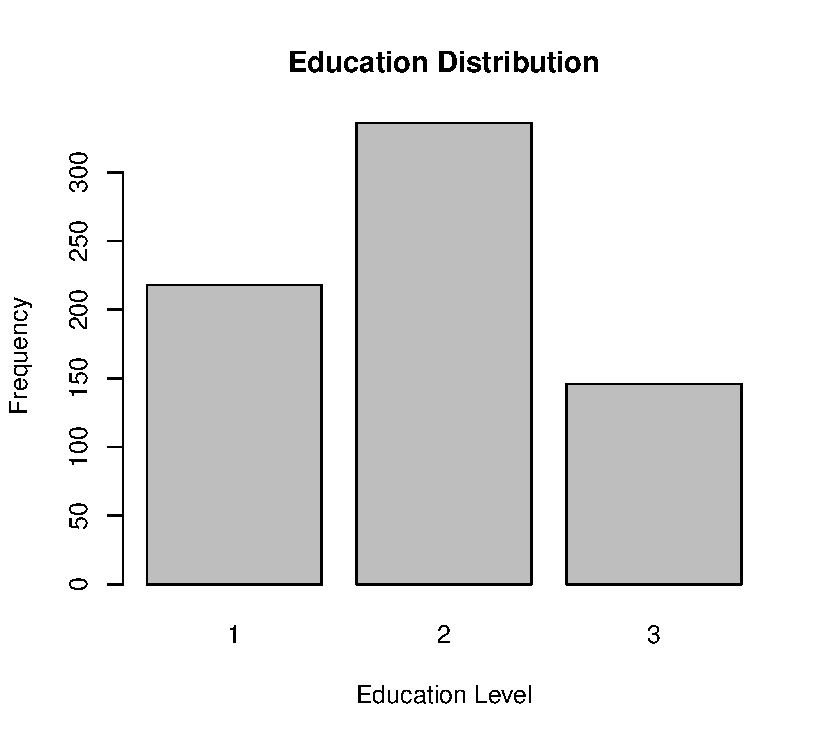
\includegraphics[scale=0.6]{Rplot2.pdf}
	\end{column}
	
	\begin{column}{0.4\textwidth}
		\begin{block}{.}
A plot of the histogram shows that the most of the caregivers on average had attained Secondary school education.
		\end{block}
	\end{column}
\end{columns}
\end{frame}
\subsection{Ordinal logistic Regression model}
\textbf{Ordinal Logistic regression Model}
\begin{knitrout}
	\definecolor{shadecolor}{rgb}{0.969, 0.969, 0.969}\color{fgcolor}\begin{kframe}
		\begin{alltt}
			\hlcom{# Fit an ordinal logistic regression model}
			\hlstd{model} \hlkwb{<-} \hlkwd{polr}\hlstd{(depression} \hlopt{~} \hlstd{age_participant} \hlopt{+} \hlstd{age_patient} \hlopt{+}
			\hlstd{marital_status} \hlopt{+} \hlstd{education} \hlopt{+} \hlstd{income_ksh} \hlopt{+} \hlstd{social_support,}
			\hlkwc{data} \hlstd{= df,}\hlkwc{Hess}\hlstd{=}\hlnum{TRUE}\hlstd{)}
		\end{alltt}
	\end{kframe}
\end{knitrout}
\begin{knitrout}
	\definecolor{shadecolor}{rgb}{0.969, 0.969, 0.969}\color{fgcolor}\begin{kframe}
		\begin{alltt}
			\hlcom{# Print the model summary}
			\hlcom{#model}
			\hlkwd{summary}\hlstd{(model)}
		\end{alltt}
		\begin{verbatim}
			## Call:
			## polr(formula = depression ~ age_caregiver + age_patient + marital_status + 
			##     education + income_ksh + social_support, data = df, Hess = TRUE)
			## 
			## Coefficients:
			##                      Value Std. Error t value
			## age_caregiver   -0.0052639   0.006954  0.7569
			## age_patient     -0.0008122   0.003406  0.2385
			## marital_status   0.0758508   0.089496 -0.8475
			## education        0.0496053   0.095367 -0.5201
			## income_ksh       0.0133679   0.018344 -0.7287
			## social_support  -0.0563137   0.149247  0.3773
			## 
			## Intercepts:
			##                  Value   Std. Error  t value
			## None|Mild       -1.3819  0.3918    -3.5275
			## Mild|Moderate    0.1779  0.3877     0.4589
			## Moderate|Severe  1.2344  0.3906     3.1606
			## Severe|Profound  2.3874  0.4035     5.9168
			## 
			## Residual Deviance: 215.684 
			## AIC: 235.684
		\end{verbatim}
	\end{kframe}
\end{knitrout}
\begin{frame}{Estimated model}
	Let $x_1$= age of caregiver, $\ldots$ $x_6$=social\_support\\
	
	From the results, the estimated model is written as:
	
	$$\begin{adjustbox}{width=\textwidth}
		logit(P(Y \leq 1)) = -1.38 - (-0.005)x_1 - (-0.0008)x_2 - (0.076)x_3 -(0.05)x_4 -(0.013)x_5 - (-0.056)x_6
	\end{adjustbox}$$
	$$\begin{adjustbox}{width=\textwidth}
		logit(P(Y \leq 2)) = 0.18 - (-0.005)x_1 - (-0.0008)x_2 - (0.076)x_3 -(0.05)x_4 -(0.013)x_5 - (-0.056)x_6
	\end{adjustbox}$$
	$$\begin{adjustbox}{width=\textwidth}
		logit(P(Y \leq 3)) = 1.23-(-0.005)x_1 - (-0.0008)x_2 - (0.076)x_3 -(0.05)x_4 -(0.013)x_5 - (-0.056)x_6
	\end{adjustbox}$$
	$$\begin{adjustbox}{width=\textwidth}
		logit(P(Y \leq 4)) = 2.39 - (-0.005)x_1 - (-0.0008)x_2 - (0.076)x_3 -(0.05)x_4 -(0.013)x_5 - (-0.056)x_6
	\end{adjustbox}$$
\end{frame}
\begin{frame}{Interpretation of the Coefficients}
\begin{itemize}
\item 	For a unit increase in the age of a caregiver, the expected change of the value of depression in log odds scale is 0.005 given all the other variables are held constant.
	
\item 	For a unit increase in the age of the patient, the expected change of the value of depression in the log odds scale is 0.0008 given all the other variables are held constant.
	
\item 	For a unit increase in the income, the expected change in the value of depression in the odd logs scale is -0.013 given all the other variables are held constant.
	
\end{itemize}
\end{frame}

\begin{frame}{Interpretation of the Coefficients cont...}
\begin{itemize}
	\item 	A unit increase in education(i.e from primary to secondary), we would expect a 0.05 decrease in the value of depression in the log odds scale, given that all of the other variables in the model are held constant.
	
	\item A one unit increase in marital status, we would expect a 0.076 decrease in the value of depression in the log odds scale, given that all of the other variables in the model are held constant.
	
	\item A one unit increase in social support, the expected change in the value of depression in log odds scale is 0.06, given that all of the other variables in the model are held constant.
\end{itemize}
\end{frame}
\textbf{Estimation of Odds Ratios}
\begin{knitrout}
	\definecolor{shadecolor}{rgb}{0.969, 0.969, 0.969}\color{fgcolor}\begin{kframe}
		\begin{alltt}
			\hlcom{## odds ratios}
			\hlkwd{exp}\hlstd{(}\hlkwd{coef}\hlstd{(model))}
		\end{alltt}
		\begin{verbatim}
			## age_participant age_patient  marital_status education   
			##       1.0052778 1.0008126       0.9269545   0.9516049   
			## income_ksh  social_support 
			## 0.9867210          1.0579295
		\end{verbatim}
		\begin{alltt}
			\hlcom{## OR and CI}
			\hlkwd{exp}\hlstd{(}\hlkwd{cbind}\hlstd{(}\hlkwc{OR} \hlstd{=} \hlkwd{coef}\hlstd{(model), ci))}
		\end{alltt}
		\begin{verbatim}
			##                        OR     2.5 %   97.5 %
			## age_Caregiver   1.0052778 0.9916830 1.019104
			## age_patient     1.0008126 0.9941470 1.007516
			## marital_status  0.9269545 0.7776230 1.104571
			## education       0.9516049 0.7892164 1.147162
			## income_ksh      0.9867210 0.9516645 1.023043
			## social_support  1.0579295 0.7894627 1.417498
		\end{verbatim}
	\end{kframe}
\end{knitrout}
\begin{frame}{Interpretation of Odds Ratio}
\begin{itemize}
	\item \textbf{Age Caregiver:}\\
	\noindent One unit increase in age of caregiver increases the odds of being depressed by 0.5\% assuming all other variables are held constant.
	
	\item \textbf{Age Patient:}\\
	\noindent One unit increase in age of the patient increases the odds of the caregiver being depressed by 0.08\% assuming all other variables are held constant.
	
	\item \textbf{Marital Status:}\
	\noindent Caregivers who are married (compared to those who are not) have lower odds of being in a higher depression level by approximately 8.4\%, assuming all other variables are held constant.
\end{itemize}
\end{frame}
\begin{frame}{Interpretation of Odds Ratio Cont...}
	\begin{itemize}
	\item \textbf{Education:} \\
	\noindent One-unit increase in Education(say from primary to secondary)reduces the odds of the caregive being depressed by 5.9\%,  assuming all other variables are held constant.
	
	\item \textbf{Household Income:} \\
	\noindent One-unit increase in Household income reduces the odds of being in higher depression level by 1.4\% assuming all other variables are held constant.
	
	\item \textbf{Social\_Support:} \\
	\noindent Caregivers involved in social support groups (compared to those not involved) have higher odds of being in a higher depression level by approximately 5.79\%, assuming all other variables are held constant.
	\end{itemize}
\end{frame}
\section{Conclusions and Recommendations}
\begin{frame}{Summary and Conclusions}
	\begin{block}{Summary}
$\bullet$ Significant depression predictors were identified.\\
$\bullet$ Estimation and interpretation of the coefficients were done.\\
$\bullet$ Determination and interpretation of the odds ratios were done.
	\end{block}
\begin{block}{Conclusions}
$\bullet$ The age of caregiver, Household income, level of education, Marital status of the caregiver and social support are significant in determining the depression severity of cancer caregivers while the age of the patient was found to be insignificant.\\

$\bullet$ The ordinal logistic regression model fits our dataset.

\end{block}
\end{frame}

\begin{frame}{Recommendations}
\begin{enumerate}
\item Kenya National Bureau  of Statistics to conduct research and store data on Depression for future research.

\item Government through state departments should develop interventions to provide tailored support to cancer caregivers. 

\item Interventions should address the financial challenges faced by cancer caregivers in rural areas.
\end{enumerate}
\end{frame}
\begin{frame}{References}
	\begin{enumerate}
\item Jain G., Roy A., Harikrishnan V., Yu S., Dabbous O. and Lawrence, C. (2013), Patient-Reported Depression Severity Measured by the PHQ-9 and Impact on Work Productivity, \emph{Journal of Occupational and Environmental Medicine}, 55(3), 252-258.
\item Kaggwa M. M., Najjuka, S. M., Nuwamanya S., Nabulo, H., and Nkola R. (2021). Depression among cancer caregivers in a rural setting.xlsx. Retrieved from
\href{https://figshare.com/articles/dataset/Depressionamongcancercaregiversinaruralsettingxlsx/doi: 10.6084/m9.figshare.14524800.v1}{figshare}

\item Laing S. S., and Jones S. M. (2016), Anxiety and Depression Mediate the Relationship between Perceived Workplace Health Support and Presenteeism, \emph{Journal of Occupational and Environmental Medicine}, 58(11), 1144-1149.

\item Leung D. Y., Mak Y. W., Leung S. F., Chiang V. C. and Loke A. Y. (2020), Measurement Invariances of the PHQ‐9 Across Gender and Age Groups in Chinese Adolescents,\emph{ Asia‐Pacific Psychiatry}, 12(3), e12381.
\seti
\end{enumerate}
\end{frame}
\begin{frame}
	\begin{enumerate}
		\conti
\item Levis B., Benedetti A. and Thombs B. D. (2019), Accuracy of Patient Health Questionnaire-9 (PHQ-9) For Screening to Detect Major Depression: Individual Participant Data Meta-Analysis,\emph{BMJ}, 365.

\item Levis B., Sun Y., He C., Wu Y., Krishnan A., Bhandari P. M. and Thombs B. D. (2020), Accuracy of the PHQ-2 Alone and in Combination with the PHQ-9 for Screening to Detect Major Depression: Systematic Review and Meta-Analysis,\emph{ JAMA}, 323(22), 2290-2300.

\item Lister K., Seale J. and Douce C. (2023), Mental Health in Distance Learning: A Taxonomy of Barriers and Enablers to Student Mental Wellbeing, \emph{Open Learning: The Journal of Open, Distance and e-Learning}, 38(2), 102-116.

\item Magtibay D. L., Chesak S. S., Coughlin K. and Sood, A. (2017), Decreasing Stress and Burnout in Nurses, \emph{The Journal of Nursing Administration}, 47(7/8), 391-395.

\seti
	\end{enumerate}
\end{frame}
\begin{frame}
	\begin{enumerate}
	\conti
\item Martin A., Sanderson K. and Cocker F. (2009), Meta-Analysis of the Effects of Health Promotion Intervention in the Workplace on Depression and Anxiety Symptoms,\emph{Scandinavian Journal of Work, Environment and Health}, 7-18.
\item  Montgomery C. D, Peck A. E and Vining G.G.(2012), Introduction to linear regression analysis, John Wiley \& Sons Inc.
\item Serpa J. G., Taylor S. L. and Tillisch K. (2014), Mindfulness-Based Stress Reduction (MBSR) Reduces Anxiety, Depression, and Suicidal Ideation in Veterans, \emph{Medical Care}, 52(12), S19-S24.
	\end{enumerate}
\end{frame}
\begin{frame}
	\begin{center}
		{\fontsize{40}{50}\selectfont Thank You!}
	\end{center}
	
\end{frame}
\end{document}